\documentclass[oneside,14pt]{extarticle}
\usepackage{cmap}
\usepackage[utf8]{inputenc}
\usepackage[english,ukrainian]{babel}
\usepackage{graphicx}
\usepackage{geometry}
\usepackage{listings}
\usepackage{float}
\usepackage{amsmath}
\usepackage{subfig}
\geometry{
	a4paper,
	left=20mm,
	right=20mm,
	top=15mm,
	bottom=15mm,
}
\lstset{
	language=c,
	tabsize=4,
	keepspaces,
	showstringspaces=false,
	frame=single,
	breaklines,
	language=C,
}
\graphicspath{ {./pictures} }
\setlength{\parindent}{4em}

\newcommand\subject{Основи програмування вбудованих систем}
\newcommand\lecturer{доцентка кафедри ПЗ\\Марусенкова Т.А.}
\newcommand\teacher{доцент кафедри ПЗ\\Крук О.Г.}
\newcommand\mygroup{ПЗ-32}
\newcommand\lab{8}
\newcommand\theme{Стандарт MISRA-С}
\newcommand\purpose{Засвоїти поняття формального інспектування та
статичного аналізу коду як інструментів перевірки програмних кодів, що
погано підлягають автоматизованому тестуванню, передусім — вбудованого
програмного забезпечення, а також навчитися реалізовувати ці техніки на
практиці вручну та за допомогою спеціальних програмних засобів}

\begin{document}
\begin{normalsize}
	\begin{titlepage}
		\thispagestyle{empty}
		\begin{center}
			\textbf{МІНІСТЕРСТВО ОСВІТИ І НАУКИ УКРАЇНИ\\
				НАЦІОНАЛЬНИЙ УНІВЕРСИТЕТ "ЛЬВІВСЬКА ПОЛІТЕХНІКА"}
		\end{center}
		\begin{flushright}
			\textbf{ІКНІ}\\
			Кафедра \textbf{ПЗ}
		\end{flushright}
		\vspace{80pt}
		\begin{center}
			\textbf{ЗВІТ}\\
			\vspace{10pt}
			до лабораторної роботи № \lab\\
			\textbf{на тему}: <<\textit{\theme}>>\\
			\textbf{з дисципліни}: <<\subject>>
		\end{center}
		\vspace{80pt}
		\begin{flushright}
			
			\textbf{Лекторка}:\\
			\lecturer\\
			\vspace{28pt}
			\textbf{Виконав}:\\
			
			студент групи \mygroup\\
			Коваленко Д.М.\\
			\vspace{28pt}
			\textbf{Прийняв}:\\
			
			\teacher\\
			
			\vspace{28pt}
			«\rule{1cm}{0.15mm}» \rule{1.5cm}{0.15mm} 2024 р.\\
			$\sum$ = \rule{1cm}{0.15mm}……………\\
			
		\end{flushright}
		\vspace{\fill}
		\begin{center}
			\textbf{Львів — 2024}
		\end{center}
	\end{titlepage}
		
	\begin{description}
		\item[Тема.] \theme.
		\item[Мета.] \purpose.
	\end{description}

    \section*{Лабораторне завдання}
    \begin{enumerate}
        \item Ознайомитися з викладеним вище теоретичним матеріалом. 
        \item Здійснити перевірку на відповідність правилам MISRA-C:2004 коду проекту, створеного у середовищі Keil uVision в рамках однієї з лабораторних робіт (на вибір студента) з дисципліни “Основи програмування вбудованих систем”. Аналіз провести вручну. Скласти звіт про помилки у вигляді табл.1.
        \item На додаток до знайдених власних помилок кодування, зумисне продумати та внести порушення тієї підвибірки правил MISRA-C: 2004, що задається номерами правил у індивідуальному завданні. Після внесення порушень проект повинен компілюватися.
        \item Для кожного згенерованого порушення правила перевірити, чи воно буде знайдене за допомогою статичного аналізатора коду. Скласти звіт за зразком, поданим у табл. 2.
        \item Перевірити, чи порушення правила може бути виявлене за допомогою налаштувань компілятора середовища Keil uVision. Скласти звіт за зразком, поданим у табл. 3.
        \item Підготувати та здати звіт про виконання лабораторної роботи.
    \end{enumerate}
    
    \section*{Індивідуальне завдання}
    Правила 20.7, 20.8, 20.10 та 20.11.

    \section*{Теоретичні відомості}
    Назвіть рекомендації щодо заповнення бланка інспектування?
    
        Вказівка імен та контактних даних осіб, які проводять інспекцію та тих, чиїй код піддається інспекції.
    Дата, коли проведена інспекція коду.
    Зазначення, чи відповідає код стандарту MISRA C, і якщо ні, то які конкретні відхилення від стандарту були виявлені.
    Виокремлення конкретних проблем, які було виявлено під час інспекції, таких як порушення стилістики коду, невідповідність вимогам безпеки тощо.
    Зазначення рекомендацій або пропозицій щодо виправлення виявлених проблем.
    Інформація про те, чи були вирішені виявлені проблеми, та які конкретні дії були проведені для виправлення.
    Додаткові коментарі або відомості, які можуть бути корисними для зрозуміння контексту і результатів інспекції.

	\section*{Хід роботи}
	
\begin{table}[H]
  \centering
  \caption{Звіт про порушення правил MISRA-C: 2004, знайдені шляхом перегляду коду}
  \label{tab:my-table}
  \renewcommand{\arraystretch}{1.5}
  \resizebox{\textwidth}{!}{
  \begin{tabular}{|p{4cm}|p{3cm}|p{7cm}|p{5cm}|}
  \hline
    Правило MISRA-C: 2004 & Ім'я файлу, номер рядка & Зміст помилки & Коректний варіант \\\hline
    8.10 & main.c & Використання extern, там, де без цього можна обійтись & Не використовувати extern \\\hline
    16.10 & main.c & Відсутність обробки помилки повернутої з функції & Обробити помилку \\\hline
    19.7 & main.c & Застосування макросів, там де можна застосувати функцію & Застосувати функцію замість макросу \\\hline
  \end{tabular}
  }
\end{table}

Код із внесеними помилками.

\begin{lstlisting}
#include <stdint.h>
#include <setjmp.h>
#include <signal.h>
#include <stdlib.h>

jmp_buf buffer;


int main(void) {
    setjmp(buffer);
    
	const int8_t *str = "123";
    int8_t number = atoi(str);
    
    exit(1);

    return 0;
}
\end{lstlisting}
	
	\begin{figure}[H]
	    \centering
	    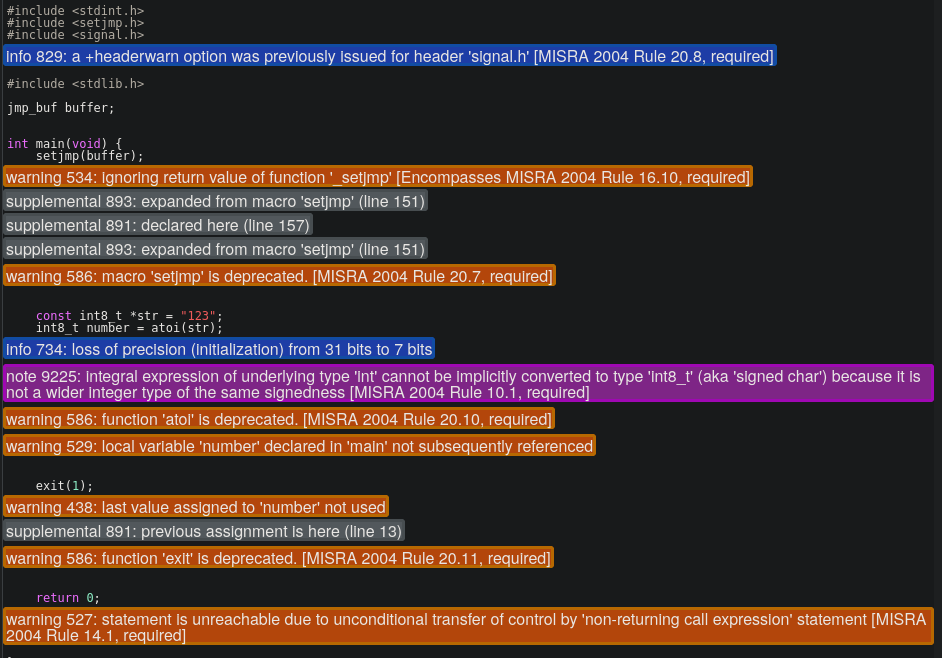
\includegraphics[scale=0.45]{1}
	    \caption{Результат статичного аналізу коду з доданими помилками.}
	\end{figure}
	
\begin{table}[H]
  \centering
  \caption{Звіт про знаходження фактів порушення правил
MISRA-C: 2004 статичним аналізатором}
  \label{tab:my-table}
  \renewcommand{\arraystretch}{1.5}
  \resizebox{\textwidth}{!}{
  \begin{tabular}{|p{4cm}|p{3cm}|p{3cm}|p{10cm}|}
  \hline
    Правило MISRA-C: 2004 & Ім'я файлу, номер рядка & Чи був знайдений аналізатором & Текст повідомлення статичного аналізатора \\\hline
    20.7 & main.c:3& + & warning 586: macro 'setjmp' is deprecated. [MISRA 2004 Rule 20.7, required] \\\hline
    20.8 & main.c:9 & + & info 829: a +headerwarn option was previously issued for header 'signal.h' [MISRA 2004 Rule 20.8, required] \\\hline
    20.10 & main.c:12 & + & warning 586: function 'atoi' is deprecated. [MISRA 2004 Rule 20.10, required] \\\hline
    20.11 & main.c:14 & + & warning 586: function 'exit' is deprecated. [MISRA 2004 Rule 20.11, required] \\\hline
  \end{tabular}
  }
\end{table}

\begin{figure}[H]
	    \centering
	    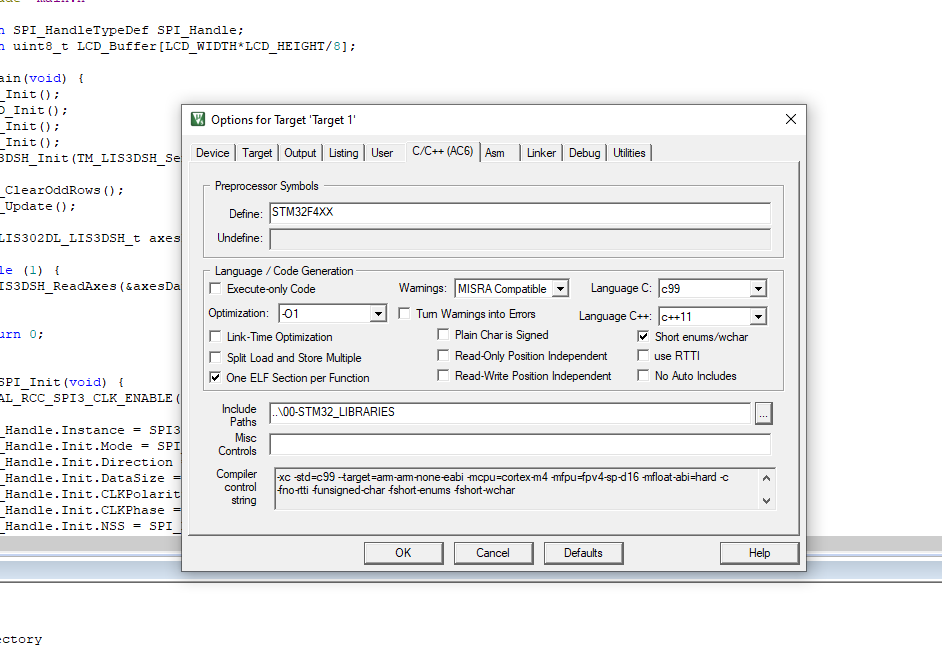
\includegraphics[scale=0.45]{2}
	    \caption{Налаштування Keil.}
	\end{figure}
	
	\section*{Висновки}
	Під час виконання лабораторної роботи я засвоїв поняття формального інспектування та статичного аналізу коду як інструментів перевірки програмних кодів, що погано підлягають автоматизованому тестуванню, передусім — вбудованого програмного забезпечення, а також навчився реалізовувати ці техніки на практиці вручну та за допомогою спеціальних програмних засобів.
	    
\end{normalsize}
\end{document}
